\section{Iteration loop}\label{iteration-loop}

In section \ref{mandelbrot-set} there was mentioned that fractals are calculated
by repeating inside an iteration loop. The loop is terminated when the calculated
number of iterations equals to \emph{maxiter} or the bailout condition is reached.
In this section the calculations inside this loop will be explained.

\subsection{Single formula fractals}\label{single-formula-fractals}

The simplest 3D fractals are calculated using single fractal formula which is
build from many equations and conditions. These equations can be modifications
of Mandelbrot Set equation or can be different mathematical equations with
several conditions.

Below there are 3 examples of fractals formulas with C language code

\subsubsection{Mandelbulb Power 2}\index{Mandelbulb} \nopagebreak

This formula is modified Mandelbrot Set equation, expanded to \nth{3} dimension.
Cross section at $ z_z = 0 $ looks exactly the same as Mandelbrot Set.
\nopagebreak

\begin{tabular}{l l}
	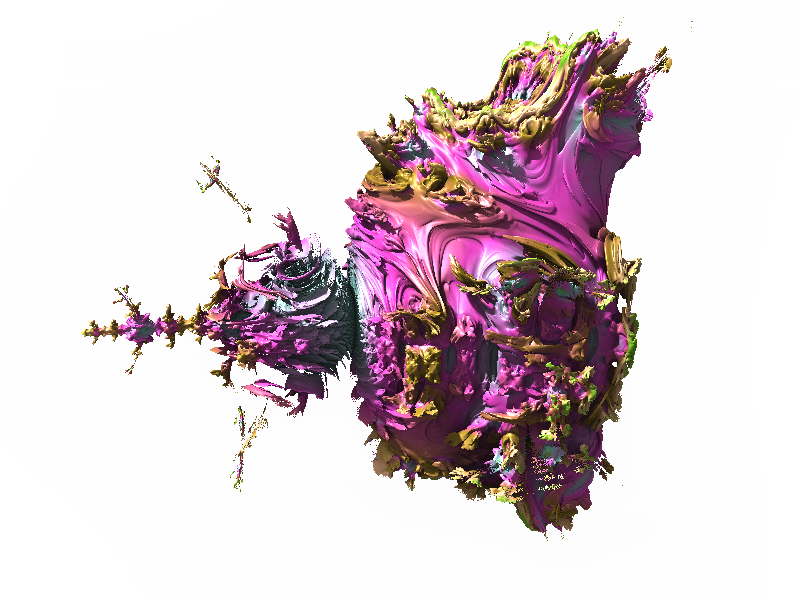
\includegraphics[width=0.3\linewidth]{img/manual/media/formula_mandelbulb_power_2}	
	& 
	\begin{minipage}[b]{0.5\linewidth}
		\begin{cppcode}
double x2 = z.x * z.x;
double y2 = z.y * z.y;
double z2 = z.z * z.z;
double temp = 1.0 - z2 / (x2 + y2);
double newx = (x2 - y2) * temp;
double newy = 2.0 * z.x * z.y * temp;
double newz = -2.0 * z.z * sqrt(x2 + y2);
z.x = newx;
z.y = newy;
z.z = newz;
		\end{cppcode}
	\end{minipage}
\end{tabular} 

\subsubsection{Menger Sponge}\index{Menger Sponge} \nopagebreak

This formula is Iterated Function System (IFS). It contains several
transformations where some of them are conditional. \nopagebreak

\begin{tabular}{l l}
	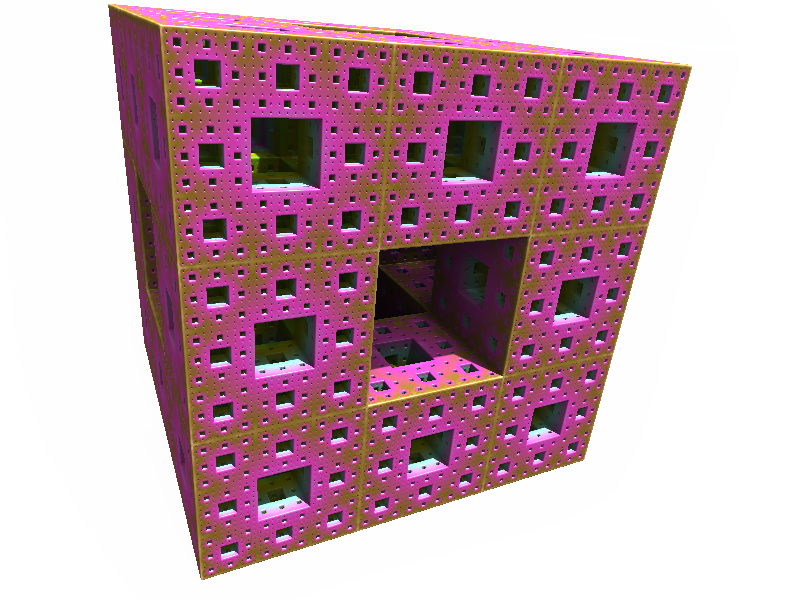
\includegraphics[width=0.3\linewidth]{img/manual/media/formula_menger_sponge.png}	
	& 
	\begin{minipage}[b]{0.5\linewidth}
		\begin{cppcode}
z.x = fabs(z.x);
z.y = fabs(z.y);
z.z = fabs(z.z);
		
if (z.x - z.y < 0.0) swap(z.x, z.y);
if (z.x - z.z < 0.0) swap(z.x, z.z);
if (z.y - z.z < 0.0) swap(z.y, z.z);
		
z *= 3.0;
		
z.x -= 2.0;
z.y -= 2.0;
if (z.z > 1.0) z.z -= 2.0;
		\end{cppcode}
	\end{minipage}
\end{tabular} 

\subsubsection{Box Fold Bulb Pow 2}
\nopagebreak

This formula is a set of different transforms and equations. It's a good example
which shows that fractal formula can be much more complicated than
\emph{Mandelbrot Set}.

First part is ``box fold''\index{transform!box fold} transform which do
transformations based on box walls. Second part is ``spherical
fold''\index{transform!spherical fold} which do transformations based on sphere.
The end of formula is the same as \emph{Mandelbulb Power 2}. \nopagebreak

\begin{tabular}{l l}
	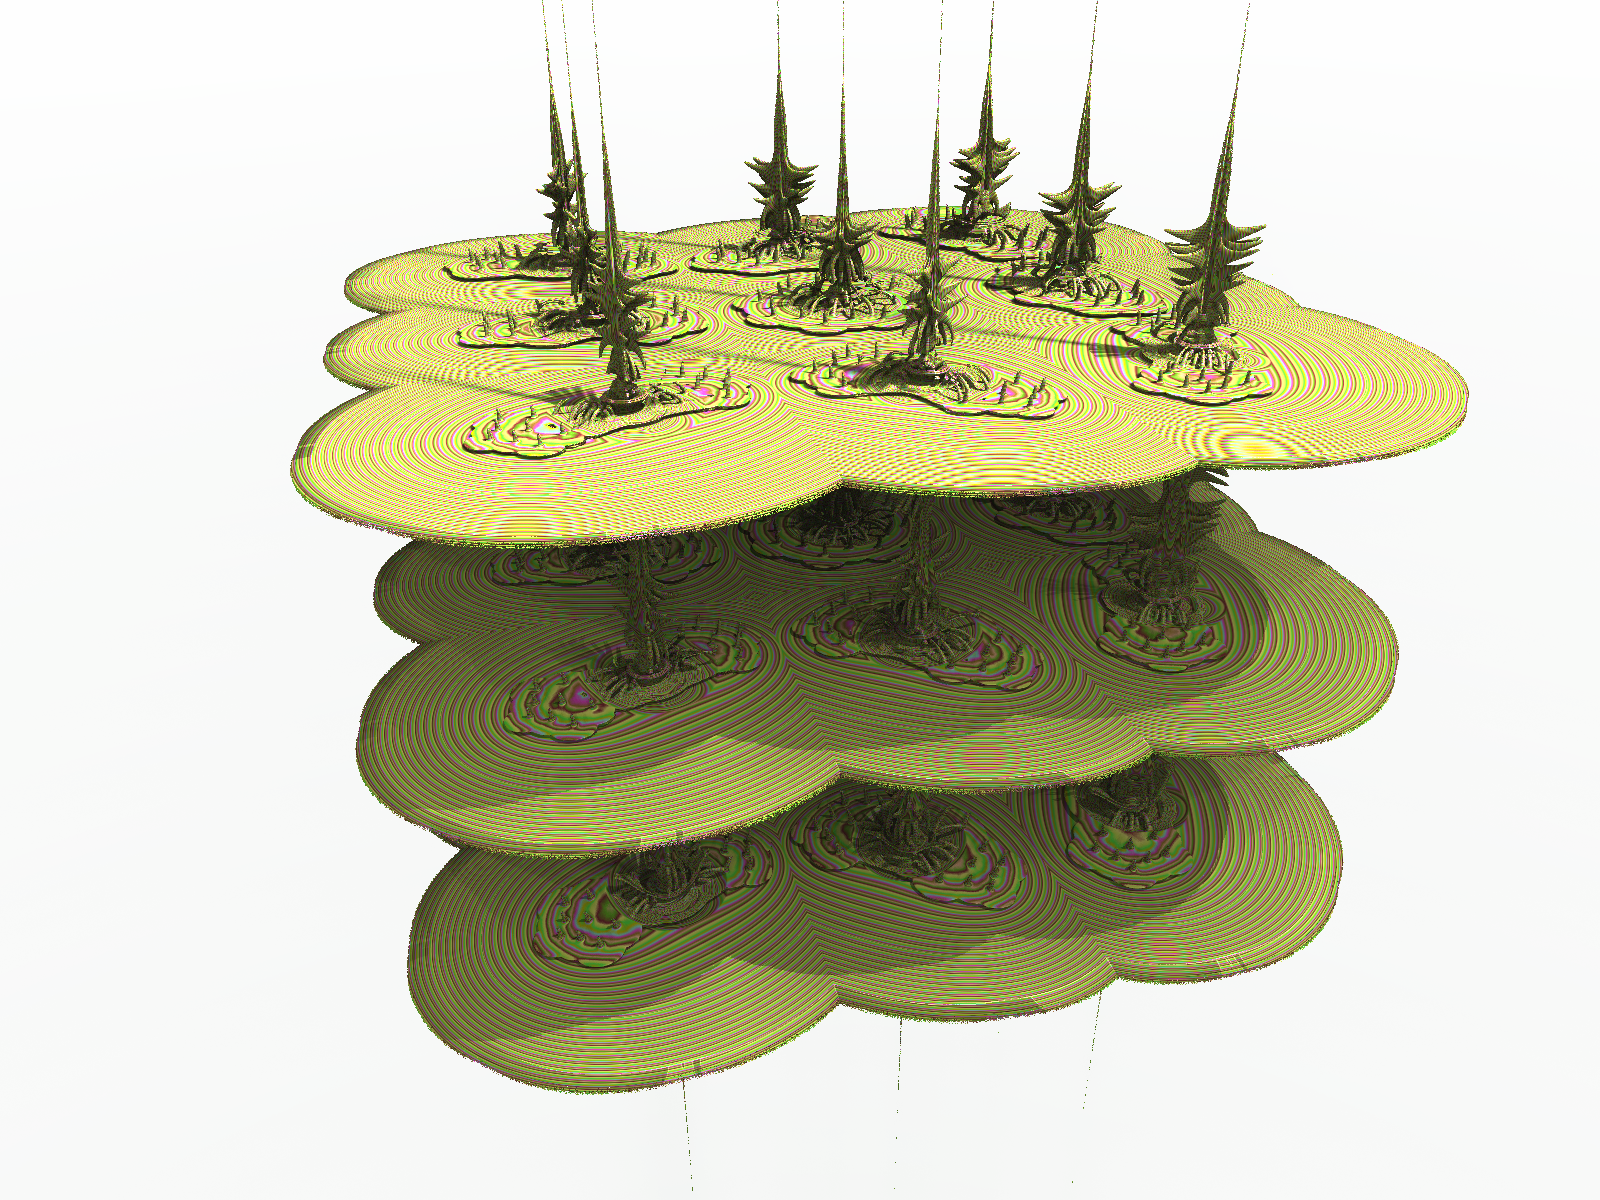
\includegraphics[width=0.3\linewidth]{img/manual/media/formula_box_fold_pwr2.png}	
	& 
	\begin{minipage}[b]{0.5\linewidth}
		\begin{cppcode}
//box fold
if (fabs(z.x) > fractal->foldingIntPow.foldFactor)
	z.x = sign(z.x) * fractal->foldingIntPow.foldFactor
		 * 2.0 - z.x;
if (fabs(z.y) > fractal->foldingIntPow.foldFactor)
	z.y = sign(z.y) * fractal->foldingIntPow.foldFactor
		 * 2.0 - z.y;
if (fabs(z.z) > fractal->foldingIntPow.foldFactor)
	z.z = sign(z.z) * fractal->foldingIntPow.foldFactor
		 * 2.0 - z.z;

//spherical fold
double fR2_2 = 1.0;
double mR2_2 = 0.25;
double r2_2 = z.Dot(z);
double tglad_factor1_2 = fR2_2 / mR2_2;

if (r2_2 < mR2_2)
{
	z = z * tglad_factor1_2;
}
else if (r2_2 < fR2_2)
{
	double tglad_factor2_2 = fR2_2 / r2_2;
	z = z * tglad_factor2_2;
}

//Mandelbulb power 2
z = z * 2.0;
double x2 = z.x * z.x;
double y2 = z.y * z.y;
double z2 = z.z * z.z;
double temp = 1.0 - z2 / (x2 + y2);
zTemp.x = (x2 - y2) * temp;
zTemp.y = 2.0 * z.x * z.y * temp;
zTemp.z = -2.0 * z.z * sqrt(x2 + y2);
z = zTemp;
z.z *= fractal->foldingIntPow.zFactor;
		\end{cppcode}
	\end{minipage}
\end{tabular} 

\subsubsection{Processing of single formula fractals}

Single formula fractals are processed in simple way. Calculation of fractal
formulas is repeated several times like it is showed on following
diagrams:\nolinebreak \nopagebreak

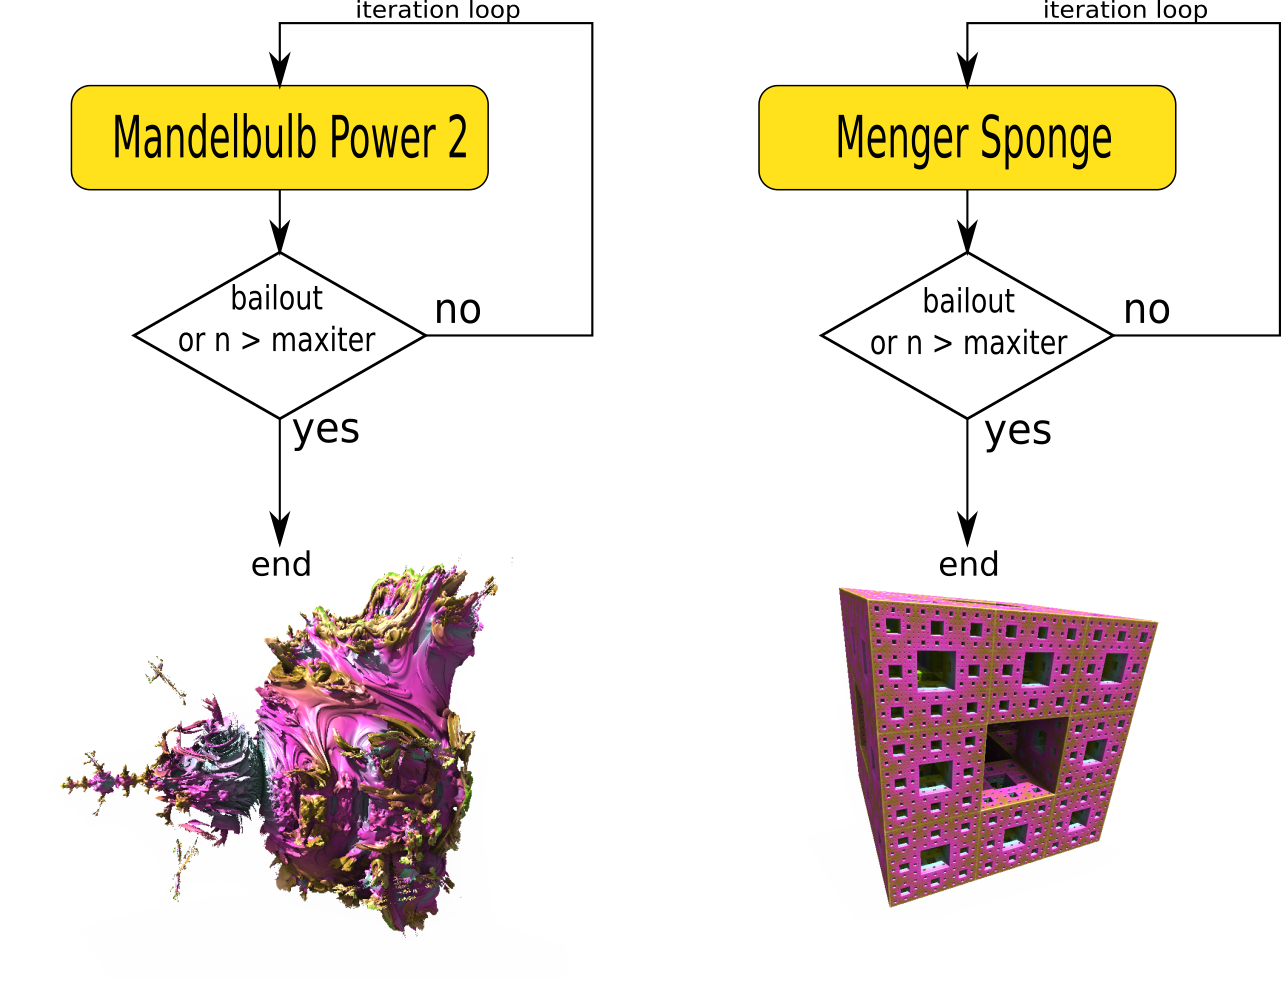
\includegraphics[width=\linewidth]{img/manual/media/iteration_loops.png}

When calculation of the iteration loop finished the result value of \emph{z} is
used to estimate distance to fractal body and to calculate color of surface.

\subsection{Hybrid fractals}\index{fractal!hybrid}

There is possible to mix different fractal formulas by alternating them, to get
new fractal shapes. That fractal are named \emph{hybrid fractals}. Mandelbulber
program already have many different fractal formulas which gives opportunity to
get very big variety of shapes. But using hybrid fractals increases
possibilities a lot.

\subsubsection{Iteration loop of hybrid fractals}

In general hybrid fractals are calculated in the same way as regular fractals.
There is iteration loop, \emph{maxiter} and \emph{bailout} condition. The
difference is in body of iteration loop. Instead of one fractal formula there
can be used different fractal formula in every iteration. There is defined
sequence which decides in which iteration the formula will be calculated. How
the sequence will work depends on following selections: \begin{itemize} \item
	Which fractal formulas are selected in formula slots \item How many iterations
	are assigned to each formula \item Range of iteration numbers where formula will
	be used \item From which fractal slot the sequence will be repeated
\end{itemize}

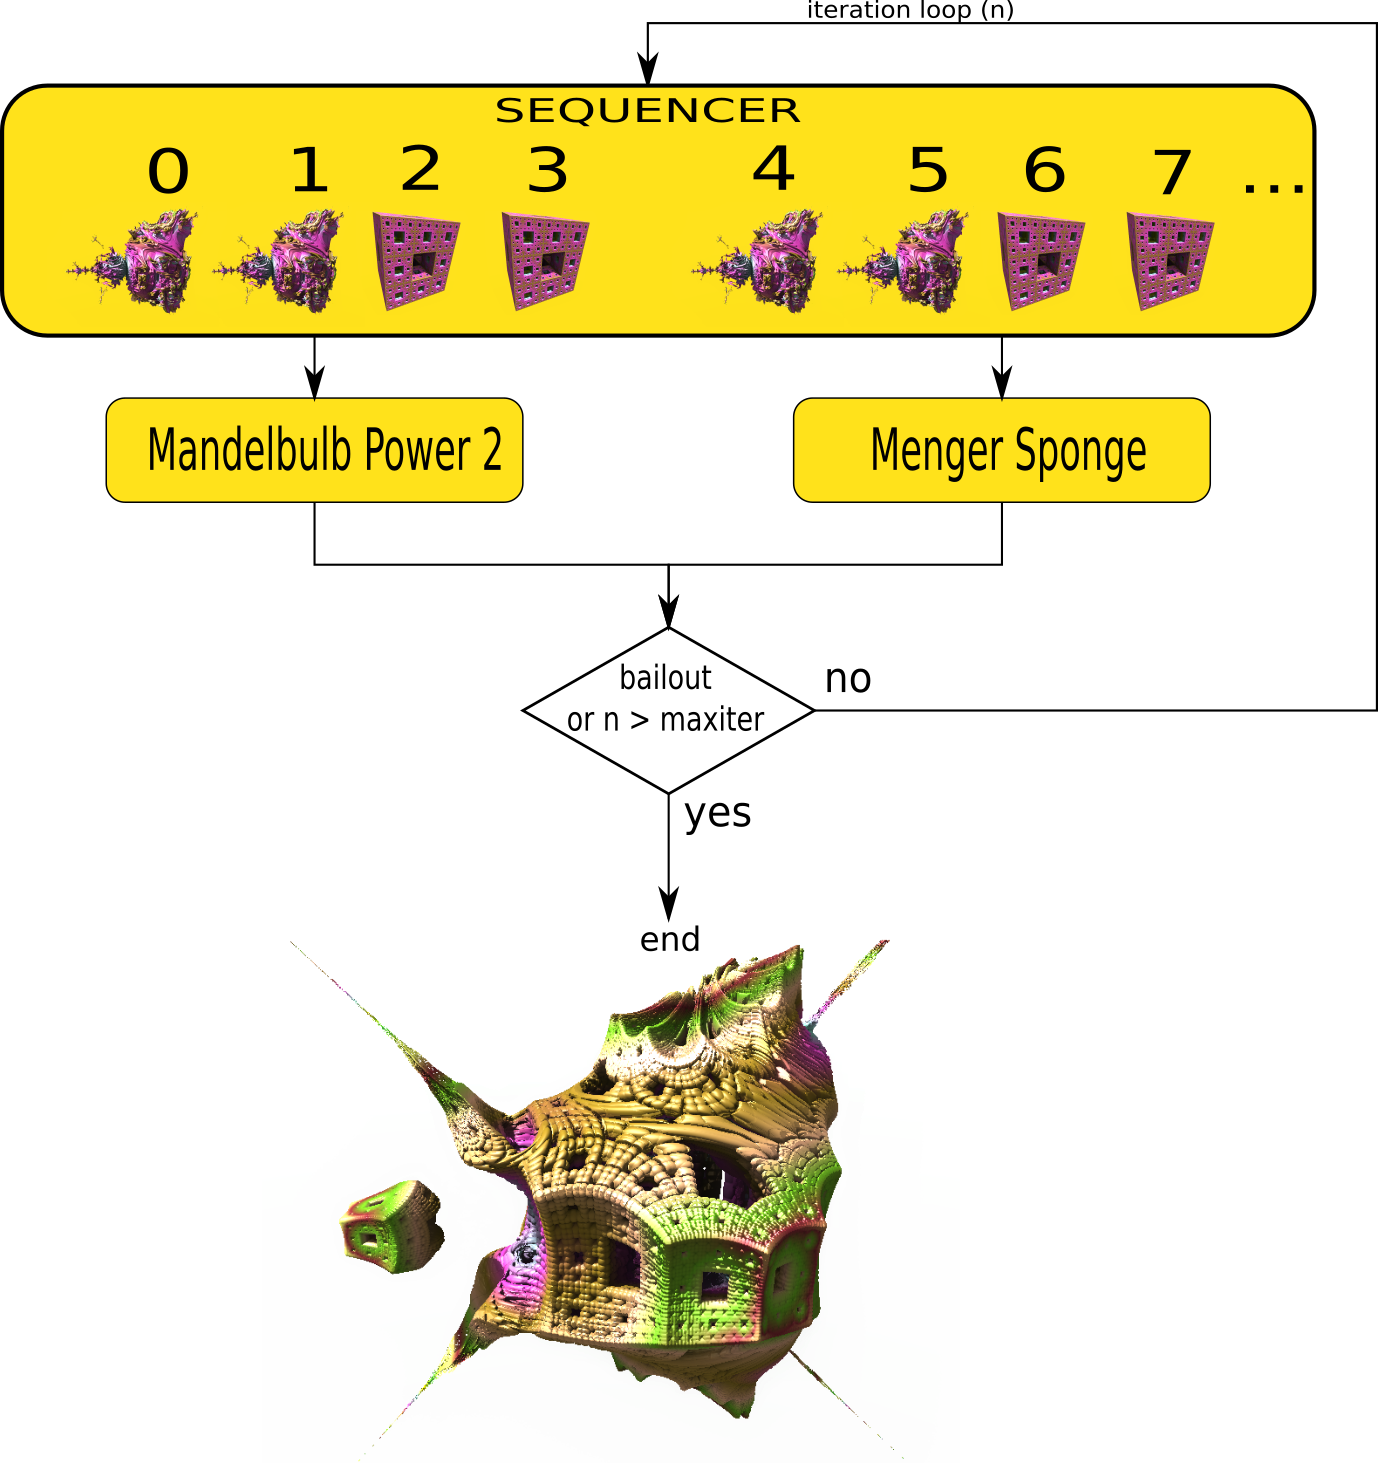
\includegraphics[width=\linewidth]{img/manual/media/iteration_loop_hybrid.png}

In Mandelbulber there is possible to define 9 different fractal formulas which
ca be alternated. Each formula is configured in separate slot (tab)

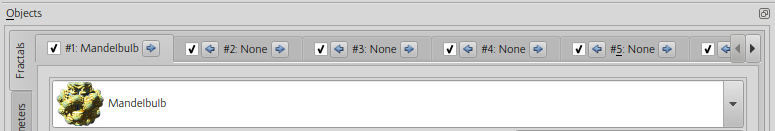
\includegraphics[width=\linewidth]{img/manual/media/fractal_tabs.png}

By default there is possible do setup fractal formula in only first slot,
because the program works in single fractal formula mode. There are two ways to
enable hybrid fractals: \begin{itemize} \item Click in any slot with number
	higher than one. The program will ask if you want to enable hybrid fractals or
	boolean mode. Select \emph{Enable hybrid fractals} \item Go to \emph{Objects} /
	\emph{Hybrid} tab. Tick \emph{Enable hybrid fractals} checkbox. \end{itemize}

After that you can switch to any slot and define fractal formulas in each slot
(if needed) like it's showed below

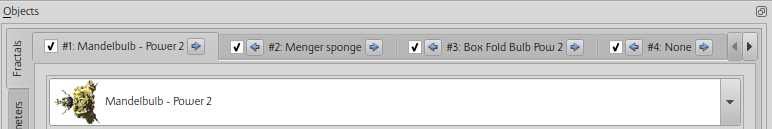
\includegraphics[width=\linewidth]{img/manual/media/fractal_tabs_with_defined_fractals.png}

There is selected \emph{Mandelbulb - Power 2} in slot \#1, \emph{Menger Sponge}
in slot \#2 and \emph{Box Fold Bulb Pow 2} in slot \#3. These formulas will be
used in next examples.

\subsubsection{One iteration for each slot}

The simplest way how hybrid fractal can be defined is to use each fractal
formula for just only one iteration in looped sequence.

I example below, there is sequence of one \emph{Mandelbulb - Power 2}, one  and
one \emph{Box Fold Bulb Pow 2}. Length of the sequence is 3, so by every 3
iterations will be repeated in the same way.

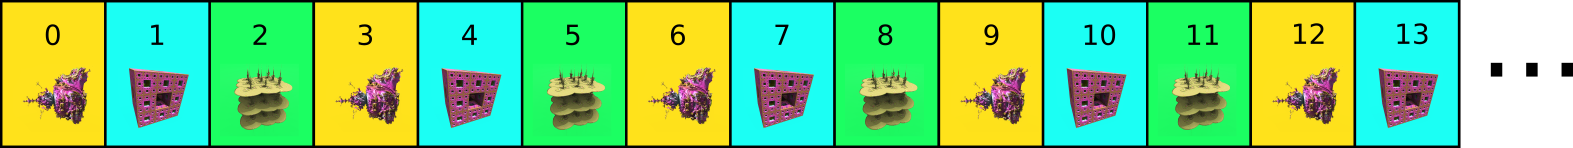
\includegraphics[width=\linewidth]{img/manual/media/iteration_loop_hybrid_sequence_1.png}

This sequence gives following shape which is a mix of properties of all 3
formulas. \nopagebreak

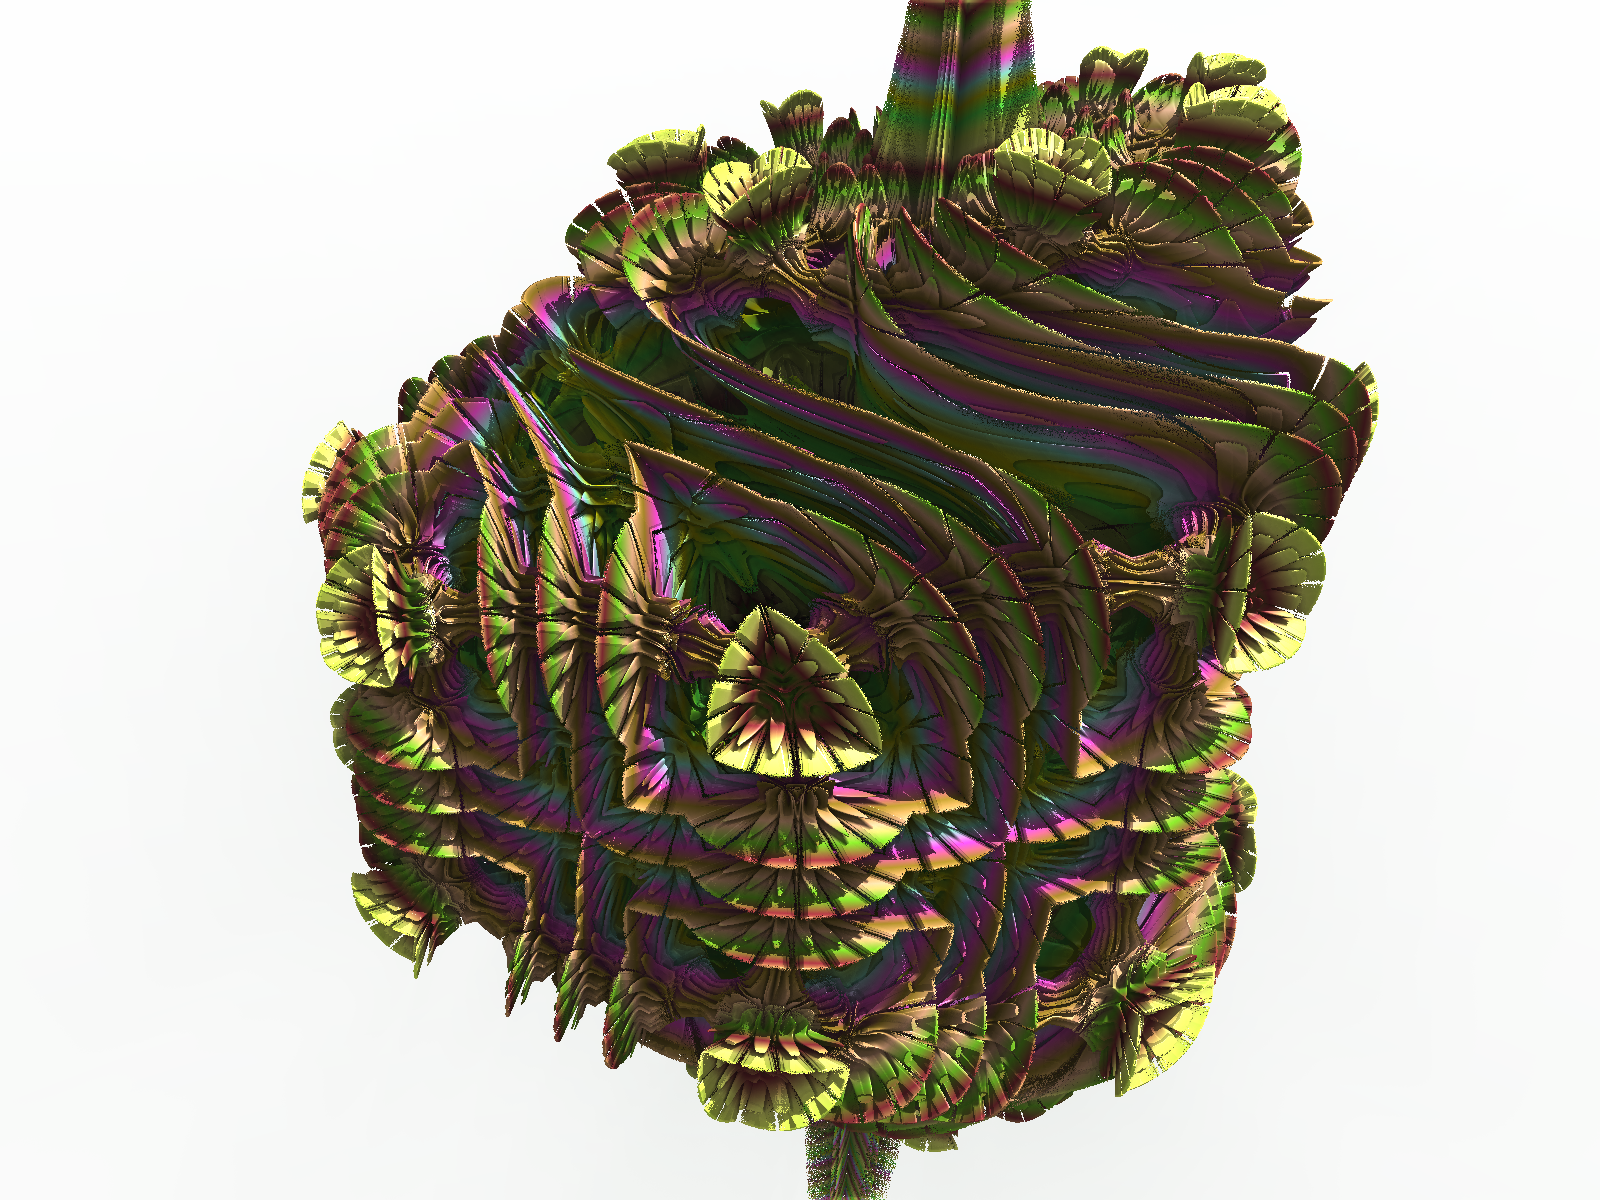
\includegraphics[width=0.7\linewidth]{img/manual/media/hybrid_sequence_example_1.png}

Because in zero iteration is used \emph{Mandelbulb - Power 2}, the general shape
of the fractal is a little similar to \emph{Mandelbulb - Power 2}

In next iteration there is used \emph{Menger Sponge} formula. Single iteration
of this formula produces this shape:

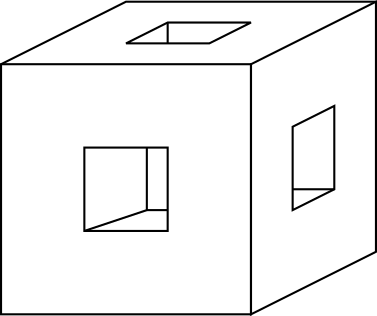
\includegraphics[width=0.2\linewidth]{img/manual/media/single_iteration_of_menger_sponge.png}

Some properties of this shape are transfered to generated shape of hybrid
fractal

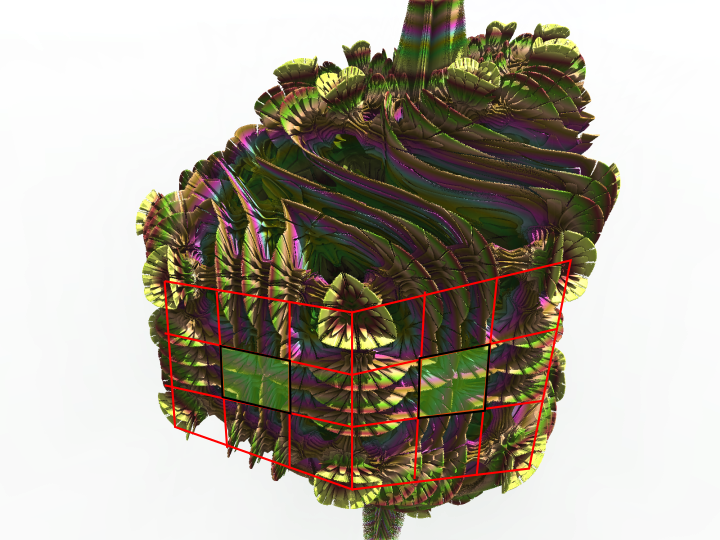
\includegraphics[width=0.5\linewidth]{img/manual/media/single_iteration_of_menger_sponge_hybrid.png}

Menger sponge shape is distorted, because \emph{Mandelbulb - Power 2} has
already deformed the space.

Third formula \emph{Box Fold Bulb Pow 2} adds leaf like features to the shape.

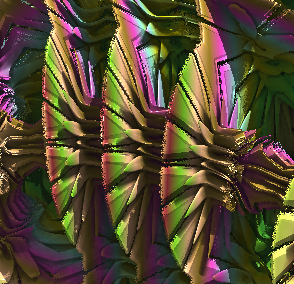
\includegraphics[width=0.4\linewidth]{img/manual/media/hybrid_sequence_example_1_leaf_shapes.png}

\subsubsection{More iterations for each slot}

In each slot there can be defined how many times fractal formula will be used in series. 
On the tab for given fractal there is parameter \emph{Iterations}. By default is set to 1. If will be increased to 2 on first and second tab, the sequence of formulas will look as following:\label{two-iterations-per-slot}

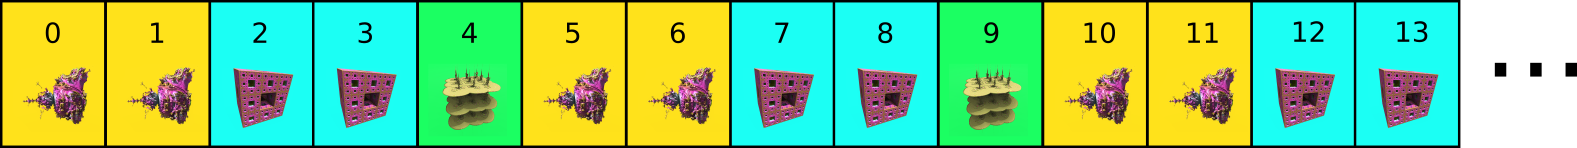
\includegraphics[width=\linewidth]{img/manual/media/iteration_loop_hybrid_sequence_2.png}

First and second formula is repeated twice and third only once. 
The fractal will get following shape.

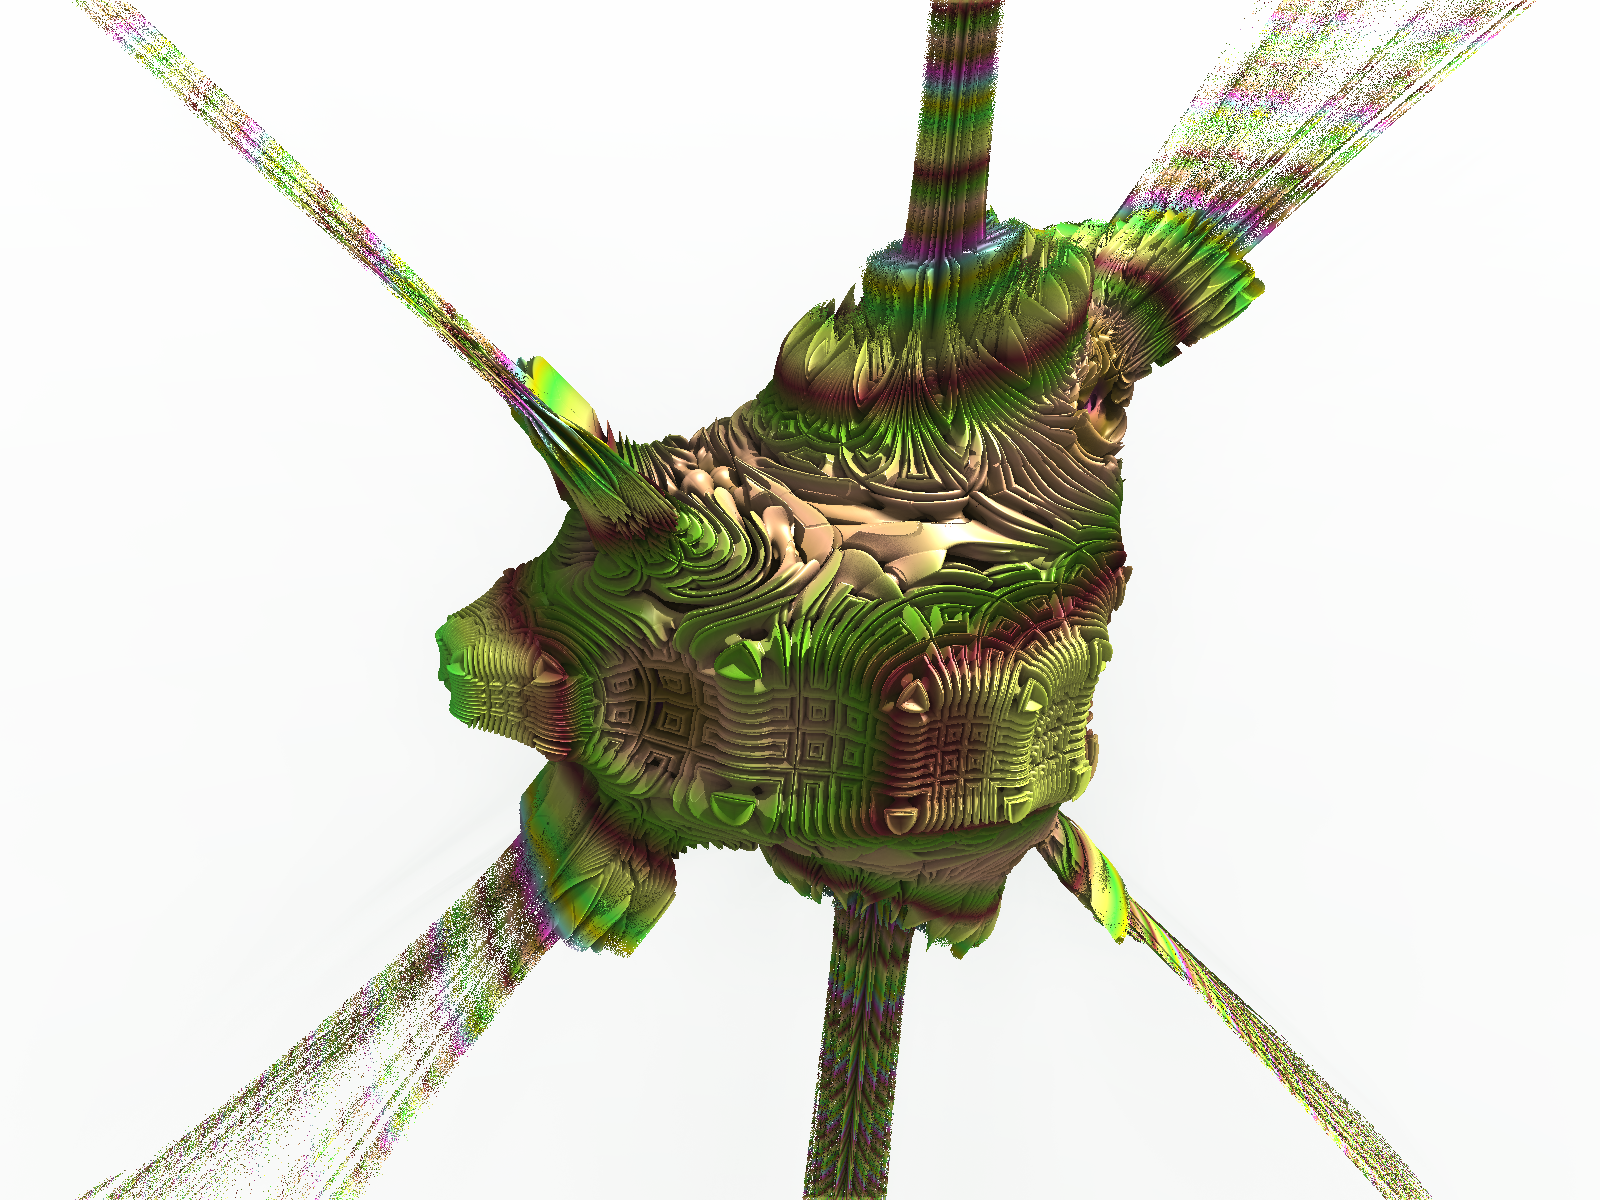
\includegraphics[width=0.7\linewidth]{img/manual/media/hybrid_sequence_example_2.png}

Because \emph{Mandelbulb - Power 2} has 2 iterations at the beginning, the shape of this formula is more visible.

If parameter \emph{Iterations} on second tab is set to 10, then \emph{Menger Sponge} is used from iteration 2 to iteration 11.

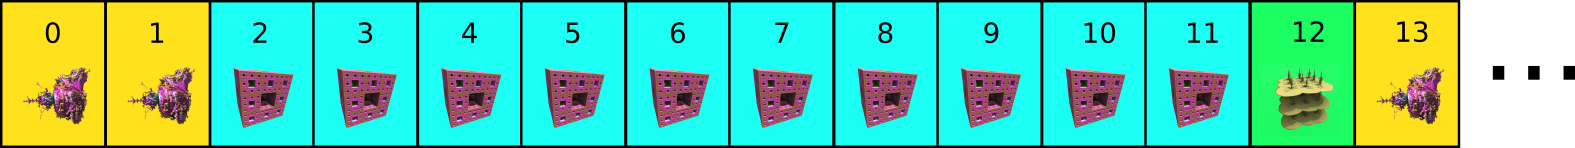
\includegraphics[width=\linewidth]{img/manual/media/iteration_loop_hybrid_sequence_3.png}

As it was before the initial shape is defined by first two iterations of \emph{Mandelbulb - Power 2}, but high number of \emph{Menger Sponge} iterations makes \emph{Menger Sponge} features very well visible.

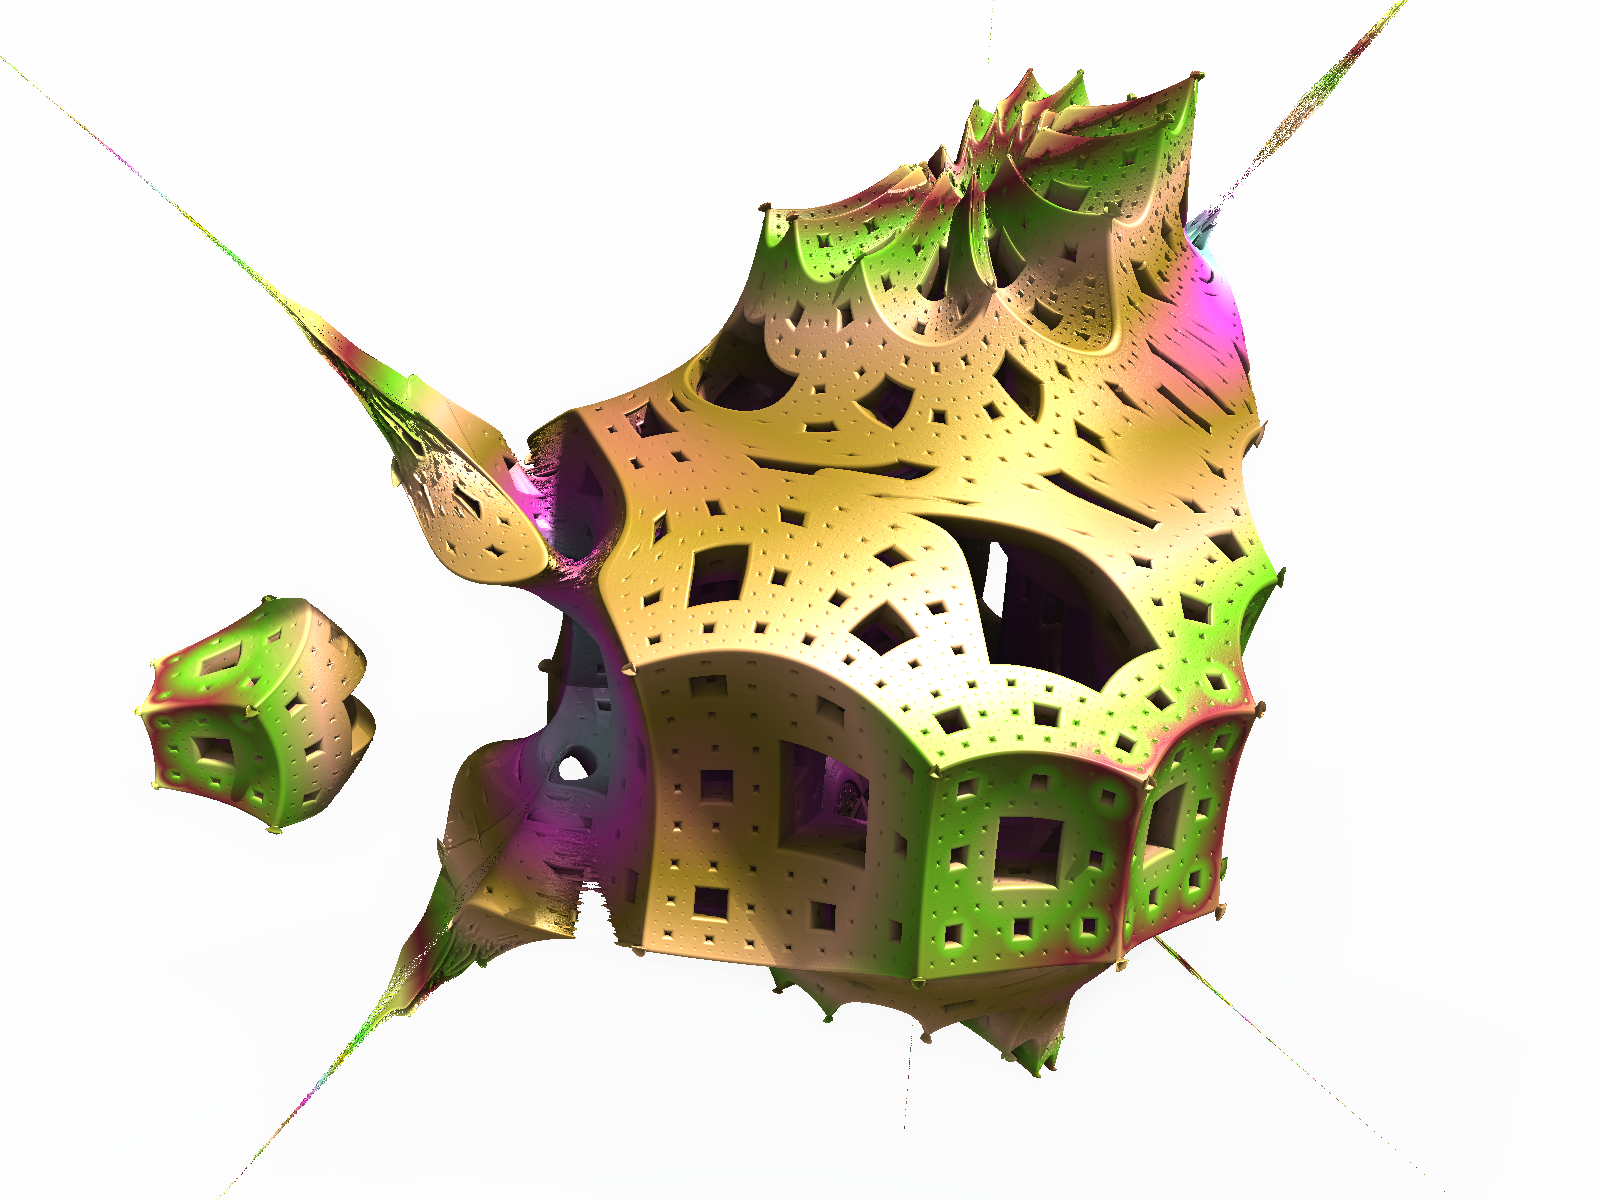
\includegraphics[width=0.7\linewidth]{img/manual/media/hybrid_sequence_example_3.png}

\subsubsection{Range of iterations for slot}

The sequence of fractal formulas can be more sophisticated. There is possible to define range of iterations on which given formula will be used.

In the example below, on the second formula slot with \emph{Menger Sponge} range of iterations was from 4 to 250. On each tab there are parameters \emph{Start at iteration} and {Stop at iteration} which are used to define this range.

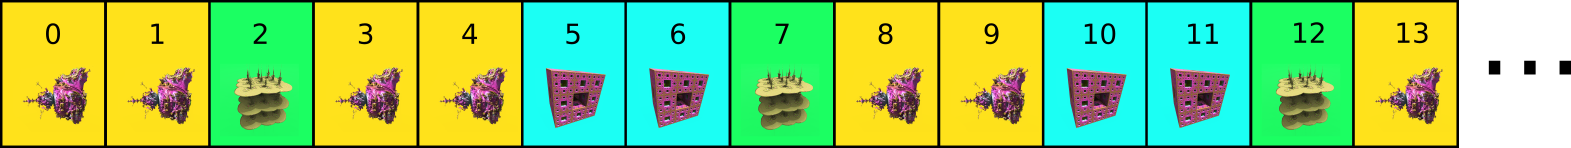
\includegraphics[width=\linewidth]{img/manual/media/iteration_loop_hybrid_sequence_4.png}

During first pass of sequence \emph{Menger Sponge} formula could be used at iterations 2 and 3. Because \emph{Start at iteration} was 4 this formula slot was skipped. During second pass of sequence \emph{Menger Sponge} formula was used at iterations 5 and 6 which were already in defined range of iterations.

The shape of fractal is following:\nopagebreak

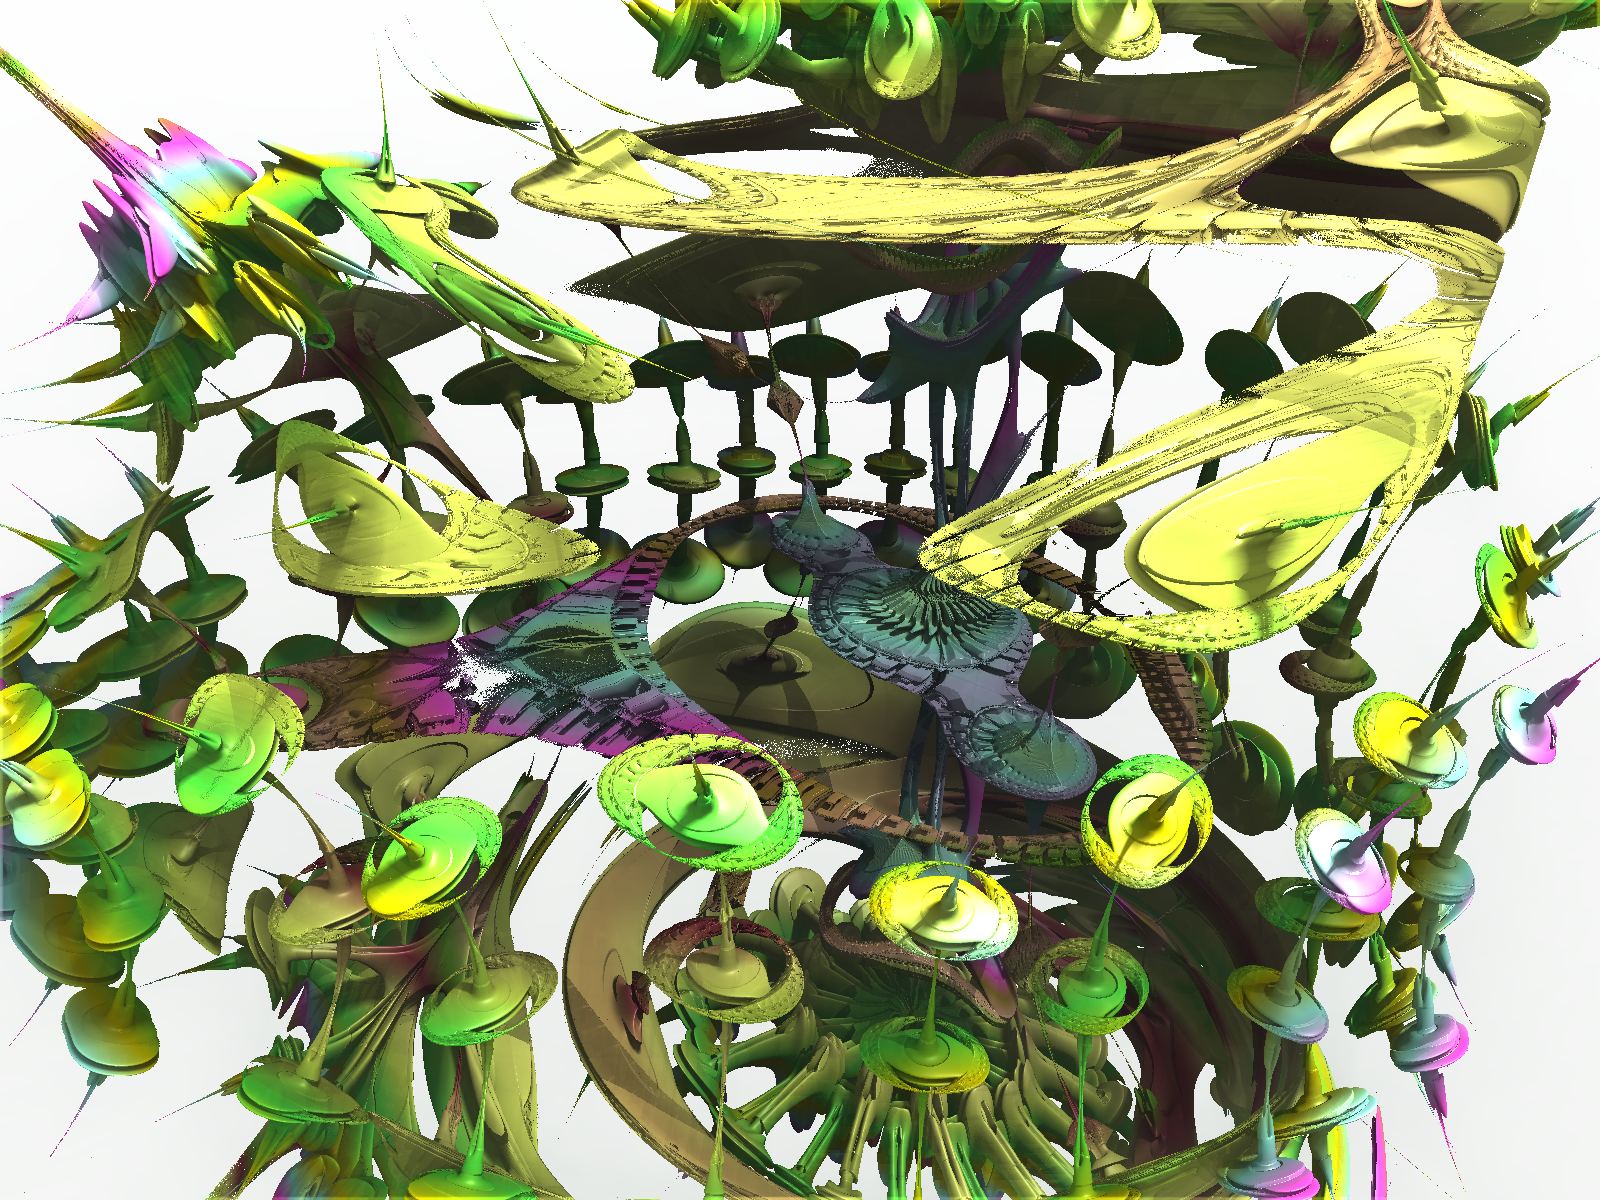
\includegraphics[width=0.7\linewidth]{img/manual/media/hybrid_sequence_example_4.png}

Because iteration number 2 is \emph{Box Fold Bulb Pow 2} formula the shape of it much more visible.

\subsubsection{Changed order in sequence}

The order of fractal formulas can be easily changed. Each fractal tab has buttons with arrows

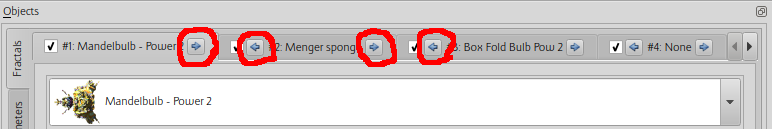
\includegraphics[width=\linewidth]{img/manual/media/fractal_tabs_with_defined_fractals_arrows.png}

Pressing of these buttons causes swapping of fractal tabs.

Example based on first case showed in section \ref{two-iterations-per-slot}:  Swapped \emph{Mandelbulb - Power 2} and \emph{Menger Sponge} gives following sequence 

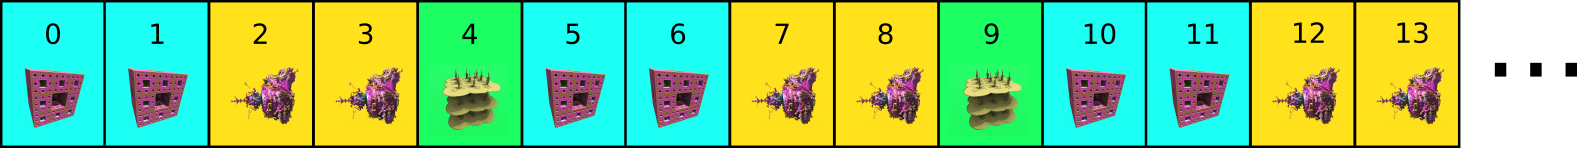
\includegraphics[width=\linewidth]{img/manual/media/iteration_loop_hybrid_sequence_5.png}

As it is visible on image below, the shape of the fractal is completely different.\nopagebreak

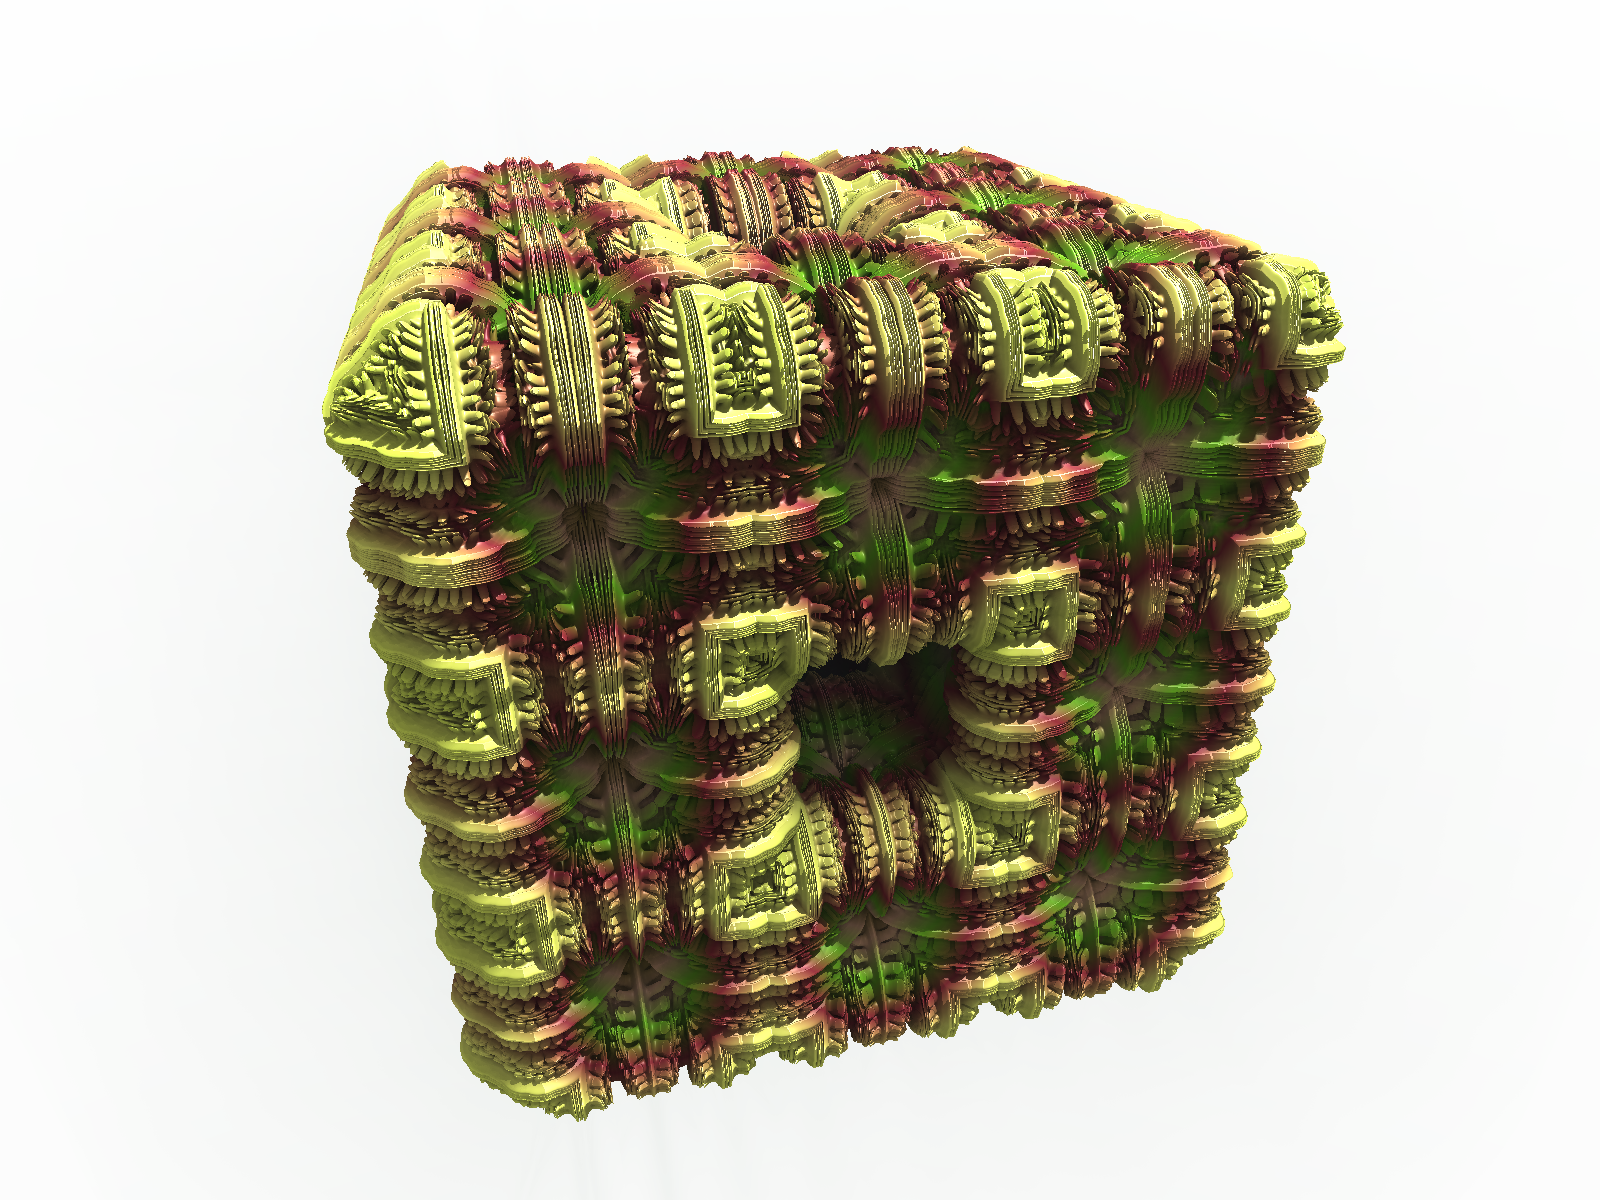
\includegraphics[width=0.7\linewidth]{img/manual/media/hybrid_sequence_example_5.png}

Even if are used the same fractal formulas and with the same number of iterations per slot, the shape strongly depends on order of formulas. Now first \emph{Menger Sponge} formula gives initial shape of fractal and \emph{Mandelbulb - Power 2} just only modifies details.
